\documentclass[12pt,openright,oneside,a4paper,english,french,spanish,brazil,nohyperref]{abntex2}

% --- Importações Padrão do Template ---
% =========================================================
% PACOTES FUNDAMENTAIS E IDIOMA
% =========================================================
\usepackage[T1]{fontenc}        % Seleção de códigos de fonte.
\usepackage[utf8]{inputenc}     % Codificação do documento (conversão automática de acentos)
\usepackage[brazil]{babel}      % Idioma do documento (traduções de "Chapter" para "Capítulo")
\usepackage{lmodern}            % Usa a fonte Latin Modern (alta qualidade em PDF)
\usepackage{textcomp}           % Símbolos complementares
\usepackage{bold-extra}         % Permite negrito e itálico/small-caps simultâneos simultaneamente

% =========================================================
% ESTRUTURA, MARGENS E LAYOUT (Padrão ABNT)
% =========================================================
% Configuração cravada de margens ABNT (3cm esq/sup, 2cm dir/inf)
\usepackage[left=3cm,top=3cm,right=2cm,bottom=2cm]{geometry}
\usepackage{setspace}           % Permite o comando \onehalfspacing (espaçamento 1.5 padrão ABNT)
\usepackage{indentfirst}        % Indenta obrigatoriamente o primeiro parágrafo de cada seção
\usepackage{lastpage}           % Conta o total de páginas (usado em fichas catalográficas e rodapés)
\usepackage{multicol} % Permite usar o ambiente \begin{multicols}


% =========================================================
% TABELAS E PÁGINAS COMPLEXAS
% =========================================================
\usepackage{longtable}          % Tabelas que quebram em várias páginas (essencial para roteiros)
\usepackage{tabularx}           % Tabelas com largura de coluna auto-ajustável (\begin{tabularx}{\textwidth})
\usepackage{makecell}           % Permite quebras de linha manuais dentro de células de tabela
\usepackage{pdflscape}          % Permite girar páginas específicas para modo paisagem
\usepackage{eso-pic}            % Inserção de imagens de fundo (marcas d'água, capas customizadas)

% =========================================================
% GRÁFICOS, CORES E FLUTUANTES
% =========================================================
\usepackage{graphicx}           % Inclusão de imagens e gráficos
\usepackage{subcaption}         % Permite subfiguras (1a, 1b, etc)
\usepackage{xcolor}             % Suporte a cores mais avançado que o antigo pacote 'color'
\usepackage{float}              % Controle rígido de flutuantes (permite o uso do [H] para fixar tabelas/figuras)
\usepackage{placeins}           % Fornece o \FloatBarrier para impedir que imagens invadam outras seções

% =========================================================
% UNIDADES E MATEMÁTICA
% =========================================================
\usepackage{units}              % Formatação padronizada de unidades de medida
% =========================================================
% PACOTES DE MATEMÁTICA
% =========================================================
\usepackage{amsmath}    % Resolve o seu erro atual (ambientes matemáticos)
\usepackage{amsfonts}   % Fontes matemáticas avançadas
\usepackage{amssymb}    % Símbolos matemáticos adicionais

% =========================================================
% MICROTIPOGRAFIA E AJUSTES FINOS
% =========================================================
\usepackage{microtype}          % Resolve 90% dos problemas de justificação (overfull/underfull hbox)
\setlength{\emergencystretch}{2em} % Dá uma folga extra para o LaTeX não jogar palavras para fora da margem
\setlength{\parindent}{1.25cm}  % Define o recuo exato do parágrafo no padrão ABNT (1.25cm a 1.5cm)

% =========================================================
% CITAÇÕES ABNT E REFERÊNCIAS
% =========================================================
% Backref DEVE vir antes do hyperref (mostra em quais páginas a referência foi citada)
\usepackage[brazilian,hyperpageref]{backref} 
% Pacote oficial de citações ABNT em formato alfabético (AUTOR, Ano)
\usepackage[alf]{abntex2cite}   

% =========================================================
% HYPERLINKS (SEMPRE O ÚLTIMO PACOTE A SER CARREGADO)
% =========================================================
\usepackage{hyperref}           % Cria links clicáveis no PDF
\hypersetup{
    colorlinks=true,            % false = links em caixas vermelhas, true = links coloridos
    linkcolor=black,            % Cor dos links internos (Sumário, figuras, tabelas) - Preto para impressão/acadêmico
    citecolor=black,            % Cor dos links de citações [1] ou (AUTOR, 2026)
    urlcolor=blue,              % Cor dos links de internet (\url)
    bookmarksdepth=4            % Nível de profundidade dos marcadores laterais no leitor de PDF
}
\input{fixos/comandos}
\usepackage{fixos/customizacoes}

% =========================================================
% PACOTES ADICIONAIS DO PROJETO
% =========================================================
% Declarados diretamente no main para evitar erros de escopo
\usepackage{multicol}   % Para as duas colunas na lista de siglas
\usepackage{pdflscape}  % Para as tabelas rotacionadas em modo paisagem
\usepackage{tabularx}   % Para tabelas dinâmicas que ocupam toda a página
\usepackage{amsmath}    % Para as renderizações matemáticas avançadas
% =========================================================

% --- Configurações Iniciais ---
% Dados pessoais
\autor{ \small
André Melo, 
Clara Nunes, 
Davi Sousa, 
Felype Carrijo, 
Gabriel Araujo, 
Giovana Silva, 
Giovanni Ferreira, 
Guilherme Mendes, 
Marco Roman, 
Matheus Pinheiro, 
Matheus Szervinsk, 
Pamela Castro, 
Paola Nascimento, 
Pedro Almeida, 
Pedro Côrtes, 
Rodrigo Barbosa, 
Thiago Silva
}
\curso{}

% Dados do trabalho
\titulo{Ratobô}
\data{2026}
\palavraChaveUm{Projeto Integrador de Engenharia 1}
\palavraChaveDois{Faculdade UnB Gama}
% Dados da orientacao
\orientador{Prof. Diogo Caetano Garcia}
\coorientador{Prof. Juliana Petrocchi Rodrigue, Prof. Hilmer Rodrigues Neri, Prof. Lui Txai Calvoso Habl e Prof. Bruno Luiz Pereira}

% % Dados para a ficha catalográfica
% \cdu{02:141:005.6}

% % Dados da aprovação do trabalho
% \dataDaAprovacao{01 de junho de 2013 -- Data da aprovação do trabalho}
% \membroConvidadoUm{Titulação e Nome do Professor Convidado 01}
% \membroConvidadoDois{Titulação e Nome do Professor Convidado 02}

\input{fixos/informacoes}
\input{fixos/setup}

\begin{document}

\frenchspacing

% ----------------------------------------------------------
% ELEMENTOS PRÉ-TEXTUAIS
% ----------------------------------------------------------
\imprimircapa
\imprimirfolhaderosto*{}

\input{fixos/fichaCatalografica}

\begin{resumo}

Este documento apresenta o desenvolvimento do Ratobô, um robô da categoria Micromouse projetado com o objetivo de mapear e resolver 
fisicamente labirintos de dimensões 4x4, 8x8 e 16x16 de maneira autônoma, integrado a uma aplicação web para armazenamento e exibição de telemetria em tempo real. 
A metodologia aplicada engloba a gestão baseada na estrutura analítica do projeto e a divisão técnica nas áreas de eletrônica, software, estrutura e energia. 
O hardware é centralizado em um microcontrolador ESP32, utilizando locomoção diferencial com motores DC N20 equipados com encoders, ponte H MX1508, e três sensores 
ultrassônicos HC-SR04, sendo alimentado por uma bateria de 12V regulada e monitorada pelo módulo INA219. No software, a navegação autônoma emprega a busca em 
profundidade para exploração e o algoritmo Floodfill para o retorno ,enquanto a interface web foi desenvolvida com React, Node.js e PostgreSQL, comunicando-se 
via MQTT e WebSockets. Como resultados esperados a partir da validação planejada, o sistema deve garantir que o robô conclua os percursos respeitando rigorosas restrições 
físicas, permitindo que a aplicação exiba instantaneamente métricas de desempenho como consumo, velocidade e o trajeto em um mapa dinâmico.

\vspace{\onelineskip}
\noindent
\textbf{Palavras-chaves}:  \imprimirpalavrachaveum, \imprimirpalavrachavedois
\end{resumo}

\input{fixos/listasAutomaticas}
\begin{siglas}
  \item[Fig.] Figura
  \item[Eq.] Equação
  \item[Tab.] Tabela
  \item[Ex.] Exemplo
  \item[PI] Projeto Integrador
  \item[ESP32] Espressif Systems 32-bit microcontroller 
  \item[MDF] Medium Density Fiberboard
  \item[CAD] Computer-Aided Design
  \item[EAP] Estrutura Analítica do Projeto
  \item[MER] Modelo Entidade-Relacionamento
  \item[DFS] Busca em Profundidade (Depth-First Search)
  \item[LM2596] Conversor DC-DC LM2596 (regulador)
  \item[HC-SR04] Sensor ultrassônico HC-SR04
  \item[INA219] Sensor de tensão e corrente INA219
  \item[MQTT] Message Queuing Telemetry Transport
  \item[WebSocket] Protocolo WebSocket
  \item[PWM] Modulação por Largura de Pulso
  \item[RF] Requisito Funcional
  \item[RNF] Requisito Não Funcional
  \item[MX1508] Ponte H MX1508
  \item[PlatformIO] Plataforma de desenvolvimento PlatformIO
\end{siglas}
 % Padrão ABNT: Siglas sempre ANTES do sumário
\input{fixos/indiceAutomatico}    % O Sumário fecha a etapa pré-textual

% ----------------------------------------------------------
% ELEMENTOS TEXTUAIS (Os capítulos do documento)
% ----------------------------------------------------------
\textual

\chapter[Introdução]{Introdução}

A convergência de competências multidisciplinares é o alicerce da disciplina de Projeto Integrador 1 (FGA0303), que propõe aos estudantes a resolução de problemas complexos por meio da engenharia prática. O presente trabalho detalha a concepção e implementação do sistema micromouse, projetado para navegação autônoma em ambientes labirínticos. O desafio exige a sincronização precisa entre algoritmos de tomada de decisão, processamento de sinais de sensores e uma estrutura mecânica otimizada para agilidade e estabilidade.

Historicamente, a robótica móvel autônoma encontrou seu espaço em soluções industriais de alto desempenho, porém, o acesso a tais tecnologias é frequentemente limitado por custos elevados de implementação e licenciamento. Nesse cenário, o desenvolvimento de protótipos baseados em sistemas embarcados de baixo custo, como o microcontrolador ESP32, surge como uma alternativa viável e educativa. O projeto foca em demonstrar que a eficiência na exploração de labirintos não depende exclusivamente de \textit{hardware} oneroso, mas sim da integração inteligente entre sensores ultrassônicos e controle em malha fechada.

Sob a ótica normativa, embora a legislação brasileira ainda não possua diretrizes específicas para a circulação de robôs autônomos de pequeno porte, a segurança operacional é balizada pela norma regulamentadora NR-12. Esta norma oferece os fundamentos necessários para mitigar riscos técnicos e garantir a integridade do equipamento e dos operadores. Adicionalmente, padrões internacionais como a ANSI/ITSDF B56.5-2019 e a EN ISO 3691-4:2020 servem de guia para o desenvolvimento de sistemas de segurança e navegação estáveis, elevando o rigor técnico do projeto para além do ambiente acadêmico.

A motivação para o desenvolvimento do micromouse fundamenta-se na busca por uma plataforma de telemetria superior às soluções de mercado. Ao contrário de modelos que operam de forma isolada, este projeto introduz uma interface de monitoramento em tempo real (Mission Control), capaz de registrar variáveis cinemáticas e de consumo energético via protocolo MQTT. Esta abordagem não apenas resolve o problema físico do labirinto, mas também melhora a análise de dados do percurso, justificando sua aplicação como um sistema de baixo custo, escalável e tecnicamente robusto para o estudo da robótica autônoma.
\chapter[Termo de Abertura do Projeto]{Termo de Abertura do Projeto}
\vspace{-1cm}

\section{Dados do Projeto}
\begin{description}
    \item [Nome do Projeto:] RATOBÔ
    \item [Data de Abertura:] 11/05/2026
    \item [Código:] 1-A
    \item [Patrocinador:] Universidade de Brasília (UnB)
    \item [Gerente:] Gabriel Alves de Araujo / Matrícula: 241025523 / E-mail: 241025523@aluno.unb.br / Contato: (61) 98469-7666
\end{description}

\section{Objetivos}
O objetivo principal é desenvolver um robô \textit{Micromouse} autônomo para mapear e resolver labirintos, integrado a uma aplicação web de telemetria em tempo real, sob gestão via Estrutura Analítica do Projeto (EAP).

Para fins de rastreabilidade, os objetivos específicos seguem a metodologia SMART:

\begin{description}
    \item [\textit{Specific} (Específico):] Criar um robô autônomo (máx. 25 cm) para navegar em malhas $4\times4$, $8\times8$ e $16\times16$ sem danificar a pista. Inclui interface web e banco de dados para telemetria instantânea (coordenadas, energia, velocidade, tempo e status).
    \item [\textit{Measurable} (Mensurável):] Resolução autônoma dos três labirintos, integridade dos registros de "Desafio" e "Trajeto" no banco de dados e construção de uma pista de testes física $4\times4$ (chão preto, paredes brancas de 5 cm, topos vermelhos).
    \item [\textit{Agreed} (Acordado):] Escopo e requisitos alinhados entre a equipe multidisciplinar e as competências exigidas pela disciplina de Projeto Integrador 1 (PI1).
    \item [\textit{Realistic} (Realista):] Viabilidade financeira assegurada pelo uso de componentes de baixo custo. A complexidade algorítmica é compatível com o nível técnico da equipe e com o cronograma de desenvolvimento.
    \item [\textit{Time Bound} (Limitado no Tempo):] Entregas incrementais vinculadas ao calendário acadêmico, garantindo protótipo e testes operacionais para a avaliação e entrega final na data estipulada pela disciplina.
\end{description}

\section{Mercado-Alvo}
O ecossistema foca em estudantes, professores e pesquisadores da área tecnológica:
\begin{itemize}
    \item \textbf{Estudantes (Engenharias):} Ferramenta prática de aprendizado interdisciplinar e validação de sistemas de controle.
    \item \textbf{Instituições de Ensino:} Plataforma modular \textit{open-source} para uso como recurso didático em laboratórios de automação.
    \item \textbf{Pesquisadores:} Base de hardware e simulador web para experimentação e avaliação comparativa de algoritmos de inteligência computacional.
\end{itemize}

\section{Requisitos do Sistema}
A Tabela \ref{tab:requisitos_micromouse} consolida as necessidades de negócio e restrições técnicas mapeadas para o projeto.

\begin{table}[H] 
    \centering
    \small
    \caption{Requisitos funcionais (RF) e não funcionais (RNF) do sistema Micromouse.}
    \label{tab:requisitos_micromouse}
    \renewcommand{\arraystretch}{1.3}
    \begin{tabularx}{\linewidth}{|l|l|X|}
        \hline
        \textbf{Cód.} & \textbf{Categoria} & \textbf{Descrição do Requisito} \\ \hline
        RF-01 & Navegação Autônoma & Resolver labirintos ($4\times4$, $8\times8$, $16\times16$) autonomamente, mapeando paredes e detectando o centro. \\ \hline
        RF-02 & Interface Web & Exibir telemetria em tempo real: tipo de labirinto, trajeto, bateria, velocidade, tempo e status de conclusão. \\ \hline
        RF-03 & Banco de Dados & Armazenar os dados finais de cada execução ao término do desafio. \\ \hline
        RF-04 & Histórico & Permitir consulta na aplicação web detalhando corridas armazenadas. \\ \hline
        RNF-01 & Dimensões & O robô não deve exceder 25 cm de comprimento/largura (sem restrição de altura). \\ \hline
        RNF-02 & Locomoção & Proibido voar, pular, escalar, usar combustão ou danificar o labirinto. \\ \hline
        RNF-03 & Inalterabilidade & Proibido alterar código/memória durante a corrida (exceto em falhas críticas). \\ \hline
        RNF-04 & Pista Física & Construir pista $4\times4$ (chão preto, paredes brancas de 5 cm com topos vermelhos). \\ \hline
        RNF-05 & Autoria & Desenvolvimento integral pela equipe (proibido plágio ou soluções prontas). \\ \hline
        RNF-06 & Gestão (GitHub) & Versionamento e controle de tarefas via \textit{issues} (máx. 2 membros por \textit{issue}). \\ \hline
    \end{tabularx}
\end{table}

\section{Justificativa}
O projeto consolida de forma prática os conceitos multidisciplinares da FCTE, unindo Engenharia de Software (arquitetura web e conectividade), Eletrônica (microcontroladores), Energia (eficiência) e Aeroespacial (cinemática). Além disso, preenche uma lacuna didática ao oferecer uma plataforma \textit{open-source} de baixo custo que, diferentemente de kits comerciais restritos, exige o domínio da construção do protótipo, gerando um ecossistema documentado para pesquisas em robótica universitária.

\section{Indicadores de Sucesso}
Para fins de avaliação técnica e acadêmica, estabelecem-se os seguintes indicadores:
\begin{enumerate}
    \item Índice de assertividade do mapeamento espacial nas malhas $4\times4$, $8\times8$ e $16\times16$.
    \item Tempo médio de resposta do \textit{pipeline} de telemetria (\textit{delay} WebSocket).
    \item Taxa de integridade dos pacotes persistidos no banco de dados PostgreSQL.
    \item Quantidade de colisões físicas registradas por ciclo de corrida.
    \item Erro percentual da odometria e sensores frente às dimensões reais da pista.
    \item Eficiência energética (Ah) em função da velocidade média dos motores.
    \item Índice de cobertura de testes automatizados (\textit{coverage}) alcançado.
    \item Vazão de tarefas (\textit{throughput}) medida pelo fechamento de \textit{issues} no GitHub.
\end{enumerate}
\begin{landscape}

\chapter{Equipe de Trabalho}

\begin{table}[htpb]
\begin{center}
\caption{Composição da equipe.}
\begin{tabular}{|c|c|c|c|c|c|}
\hline
\textbf{Nome} & \textbf{Matrícula} & \textbf{Curso} & \textbf{Telefone} & \textbf{E-mail} & \textbf{Atribuições}\\ \hline
Gabriel Alves de Araujo & 241025523        & Eng. de Software      & (61) 98469-7666   & 241025523@aluno.unb.br   & \textbf{Gerência}, Eletrônica\\ \hline
Matheus Pinheiro      & 241025336        & Eng. de Software      & (11) 94270-3735   & matheus2006.pinheiro@gmail.com & Software \\ \hline
Felype Gomes Ribeiro Carrijo       & 241025766        & Eng. de Software      & (61) 99557-5171   & 241025766@aluno.unb.br        & \textit{Eletrônica} \\ \hline
Thiago Ribeiro de Maceda da Silva & 241025864 & Eng. Eletronica & (61) 991331339 & tiao6450@gmail.com & Colíder da eletrônica \\ \hline
Davi Mesquita Sousa & 222006650 & Eng. de Software & (61) 99379-1536 & davimesquita.2004@gmail.com & Energia \\ \hline
André Ricardo Meyer de Melo & 231011097 & Eng. de Software & (61) 98288-0999 & andre.dedemeyer@gmail.com & Software \\ \hline
Giovana Barbosa da Silva & 221031283 & Eng. de Software & (62) 98459-1889 & barbosagiovana11@gmail.com & Estruturas \\ \hline
Giovanni Dornelas Ferreira & 232002664 & Eng. de Software & (61) 99169-8137 & giovannidornelasf@gmail.com & Software \\ \hline
Marco Antônio Araujo Roman & 241025309 & Eng. de Software & (61) 99220-6444 & 241025309@aluno.unb.br & Energia \\ \hline
Paola Nascimento & 211062713 & Eng. de Software & (61) 99135-1305 & 211062713@aluno.unb.br & Estruturas \\ \hline
Pedro Paulo Santos Almeida & 221008688 & Eng. de Software & (61) 99173-2649 & pedro991@outlook.com.br & Software \\ \hline
Rodrigo Carvalho Barbosa & 242035640 & Eng. de Software & (61) 99995-6848 & carvalhorodrigobarbosa@gmail.com & Energia \\ \hline
Guilherme Andrade Mendes & 231011391 & Eng. Eletronica & (61) 98363-5533 & guilhermemendesan@gmail.com & Colíder da eletrônica \\ \hline
Clara dos Santos Oliveira Nunes & 241038460 & Eng. de Software & (61) 98662-3435 & 241038460@aluno.unb.br & Estruturas \\ \hline
Pedro Silva Côrtes & 222006365 & Eng. aeroespacial & (61) 98415-9983 & cortespedro997@gmail.com & Gerente de estruturas \\ \hline
Pamela Pitombeira de Castro & 200059882 & Eng. de Energia & (61) 98418-9572 & pamelapc803@gmail.com & Líder de Energia \\ \hline
Matheus Ribeiro Szervinsk & 231011749 & Eng. de Software & (61) 98219-3662 & mathszer1103@gmail.com & Líder de Software \\ \hline
\end{tabular}
\end{center}
\end{table}

\begin{table}[htpb]
\begin{center}
\caption{Avaliação de desempenho da equipe.}
\begin{tabular}{|c|c|c|c|c|c|c|c|}
\hline
 & \textbf{Avaliação} & \textbf{Moti-} & \textbf{Comprome-} & \textbf{Conhecimento} & \textbf{Cumpriu} & \textbf{Comuni-} & \textbf{Gestão} \\
 \textbf{Nome} & \textbf{geral} & \textbf{vação} & \textbf{timento} & \textbf{técnico} & \textbf{prazos} & \textbf{cação} & \textbf{de conflitos} \\ \hline
Fulano & +++ & +++++ & +++++ & +++ & +++ & + & +++ \\ \hline
Beltrano & +++ &  +++ & +++ & + & +++ & +++++ & +++ \\ \hline
%  &  &  &  &  &  &  & em mais de uma linha \\\hline
Ciclano & +++++ & +++ &  +++++ & +++ & +++ & +++ & +++  \\ \hline
  &  &  &  &  &  &  &     \\ \hline
  &  &  &  &  &  &  &     \\ \hline
  &  &  &  &  &  &  &     \\ \hline
  &  &  &  &  &  &  &     \\ \hline
  &  &  &  &  &  &  &     \\ \hline
  &  &  &  &  &  &  &     \\ \hline
  &  &  &  &  &  &  &     \\ \hline
  &  &  &  &  &  &  &     \\ \hline
  &  &  &  &  &  &  &     \\ \hline
  &  &  &  &  &  &  &     \\ \hline
  &  &  &  &  &  &  &     \\ \hline
  &  &  &  &  &  &  &     \\ \hline
\multicolumn{8}{c}{\textit{Legenda}: +++++: \textit{atende às expectativas}; +++: \textit{requer pequenas melhorias}; +: \textit{requer grandes melhorias}.} 
\end{tabular}
\end{center}
\end{table}


\end{landscape}
\chapter{Projeto Conceitual do Produto}

\section{Características gerais}

\textcolor{red}{Descrever produto de forma geral. Apresentar itens teóricos sobre o projeto a serem aprofundados ou detalhados oportunamente.}

\textcolor{red}{Apresentar e explicar a Estrutura Analítica do Projeto (EAP), tomando cuidado com a legibilidade da imagem. Se necessário, coloque a EAP dentro do comando ``\textsf{\textbackslash begin\{landscape\} \textbackslash end\{landscape\}}'' para que ela seja apresentada em uma página deitada.}

\section{Estrutura}

\textcolor{red}{Apresentar desenho em CAD, indicar dimensões por lado/aresta/cota, indicar materiais utilizados e explicar o desenho e as decisões de projeto.}

\section{Descrição de \textit{hardware}}

\textcolor{red}{A descrição de \textit{hardware} no documento deve permitir que outras pessoas repliquem o produto proposto neste documento. Para isso, deve-se explicar de forma textual os principais sub-sistemas e as escolhas de projeto, além de indicar:}

\begin{itemize}
    \item \textcolor{red}{ O diagrama de blocos \cite{blockdiagram}, que oferece uma visão geral do hardware, com as principais partes do sistema e as ligações entre elas.}
    %\item A lista de materiais \cite{bom}, que facilita a montagem do sistema, indicando tudo que deve ser adquirido. Aproveitem a lista de materiais para apresentarem o orçamento dos mesmos.
    \item \textcolor{red}{ O esquemático \cite{esquematico}, que mostra as conexões elétricas entre os componentes. Deve-se indicar os componentes por nomes e símbolos, e as conexões entre eles, incluindo a pinagem dos componentes. Se o esquemático ficar muito grande, pode-se separa-lo em vários esquemáticos. A ligação em \textit{protoboard} não é considerada um esquemático adequado.}
\end{itemize}

\textcolor{red}{A Fig. \ref{fig:diagrama_blocos_e_esquematico} apresenta o diagrama de blocos e o esquemático de um circuito conversor de corrente alternada para corrente direta, a título de exemplo. Repare que o diagrama de blocos indica os subsistemas do circuito completo apresentado no esquemático.
% Comecem com o diagrama de blocos, que é mais genérico, e depois indiquem os detalhes com a lista de materiais e os esquemáticos.
}

\begin{figure}
    \centering
    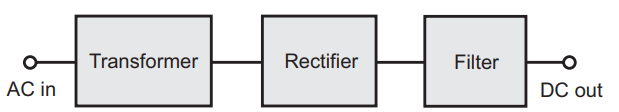
\includegraphics[width=0.5\linewidth]{figuras/Exemplo-diagrama-de-blocos.png}
    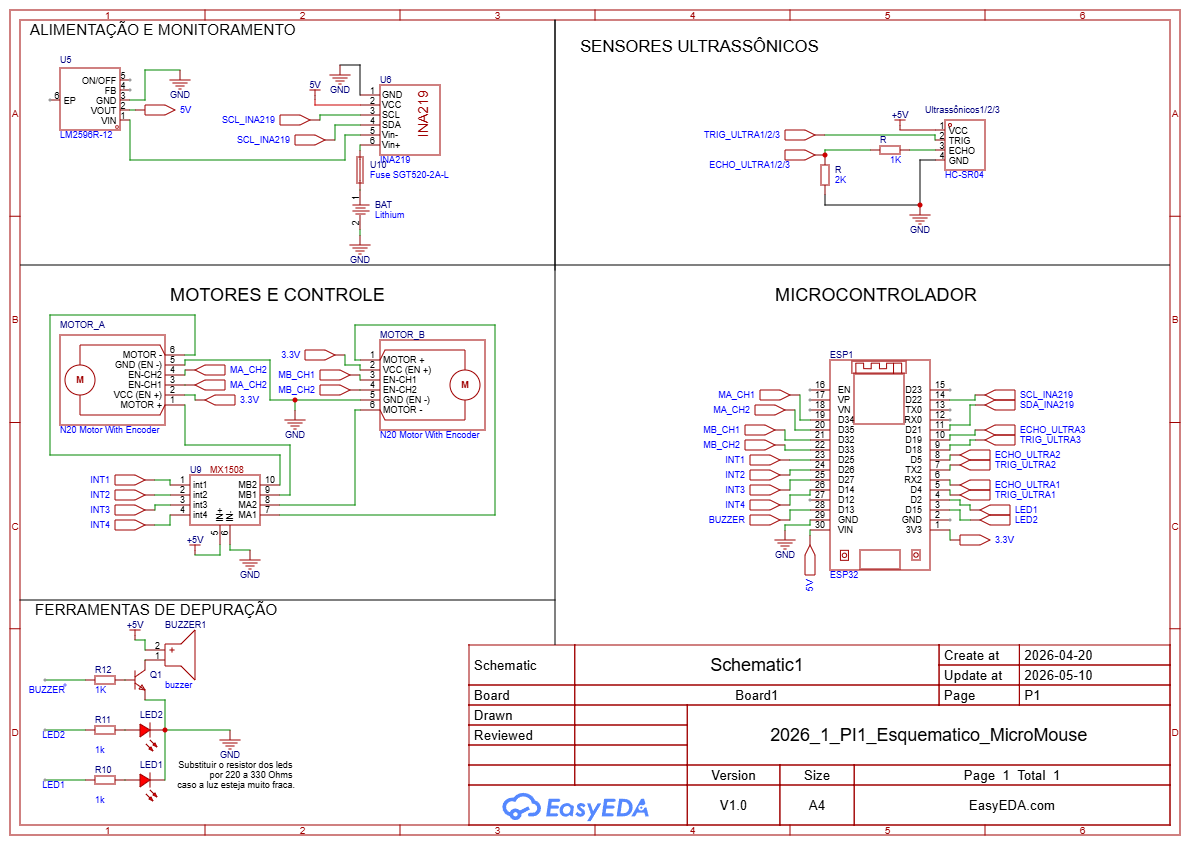
\includegraphics[width=0.5\linewidth]{figuras/Esquematico.png}
    \caption{\textcolor{red}{Diagrama de blocos e esquemático de um circuito conversor de corrente alternada para corrente direta. Extraído de \cite{block_n_schematic}.}}
    \label{fig:diagrama_blocos_e_esquematico}
\end{figure}

\section{Análise de consumo energético}

\textcolor{red}{Com relação ao consumo energético do produto desenvolvido, será necessário apresentar cálculos de consumo dos diversos componentes utilizados e explicar as decisões de projeto para atender a estas demandas.}


\section{Análise de consumo energético}

Abaixo, apresenta-se o detalhamento do consumo energético do sistema, considerando os componentes selecionados e o regime de operação previsto para o produto.

\begin{itemize}
    \item \textbf{Identificação dos Subsistemas Elétricos:} 
    O sistema é alimentado por uma bateria de 12V, cuja tensão é reduzida para o funcionamento dos demais componentes. O tempo estimado de operação contínua é de 7200 segundos (2 horas):
    \begin{itemize}
        \item \textbf{Microcontrolador (ESP32 DevKit):} 5V, 150mA, 7200s.
        \item \textbf{Atuadores (2x Motores N20):} 5V (via regulador), 240mA total, 7200s.
        \item \textbf{Sensores (Ultrassônicos):} 5V, 45mA, 7200s.
        \item \textbf{Indicadores (Buzzer e LEDs):} 5V, 40mA, 7200s.
        \item \textbf{Monitoramento (Sensor INA219):} 5V, 1mA, 7200s.
    \end{itemize}

    \item \textbf{Cálculo da Energia Consumida por Componente:} 
    Os cálculos foram realizados utilizando a fórmula $E = V \cdot I \cdot t$:
    \begin{itemize}
        \item $E_{ESP32} = 5V \times 0,150A \times 7200s = 5.400$ J
        \item $E_{Motores} = 5V \times 0,240A \times 7200s = 8.640$ J
        \item $E_{Sensores} = 5V \times 0,045A \times 7200s = 1.620$ J
        \item $E_{Indicadores} = 5V \times 0,040A \times 7200s = 1.440$ J
        \item $E_{INA219} = 5V \times 0,001A \times 7200s = 36$ J
    \end{itemize}

    \item \textbf{Estimativa do Consumo Total de Energia:} 
    A energia total consumida estimada para o ciclo é de \textbf{17.136 Joules}. Considerando o consumo médio de 476 mA, a demanda prevista para 2 horas de uso é de aproximadamente \textbf{952 mAh}.

    \item \textbf{Escolha da Fonte de Alimentação:} 
    O consumo total equivale a 4,76 Wh. A bateria selecionada (Li-ion 3x18650, 12V, 2000 mAh) fornece 24 Wh, garantindo uma margem de segurança superior a 50\%, o que é ideal para compensar perdas térmicas e picos de corrente.

    \item \textbf{Planejamento do Circuito de Alimentação:} 
    Utiliza-se o regulador de tensão \textbf{LM2596 (Step-Down)} para converter os 12V da bateria em 5V estáveis. O circuito conta com o sensor \textbf{INA219} para monitoramento de corrente e tensão, servindo como proteção contra sobrecargas.

    \item \textbf{Monitoramento via \textit{software}:} 
    O ESP32 realiza a leitura do sensor INA219 via código, permitindo acompanhar o consumo em tempo real e registrar o tempo de operação para evitar a descarga profunda da bateria.

    \item \textbf{Validação com Testes Reais:} 
    A validação compara a autonomia teórica com a real. Diferenças encontradas são atribuídas à eficiência do LM2596 (80-90\%) e dissipação por Efeito Joule nos condutores.
\end{itemize}

\section{Descrição de \textit{software}}

\textcolor{red}{Itens fundamentais:}

\begin{itemize}
    \item \textcolor{red}{ \textbf{Diagrama Atividades UML:}  descrever e explicar o fluxo do comportamento funcional do produto proposto, evidenciando, de forma clara e estruturada, como as atividades são executadas, em que ordem e sob quais condições. Esse diagrama permite compreender o funcionamento dinâmico do sistema, destacando:}

    \begin{itemize}
        \item \textcolor{red}{ os principais atores (usuários ou sistemas externos) envolvidos no processo;
        \item as atividades de negócio realizadas por cada ator ou pelo próprio sistema;
        \item os insumos (entradas) necessários para a execução das atividades;
        \item os resultados (saídas) gerados ao longo do fluxo;
        \item os pontos de decisão, paralelismo e sincronização das atividades;
        \item Entre as notações mais relevantes, destacam-se o estado iniciail e final, atividades, nós de decisão e junção, barras de bifurcação, Raias (\textit{swimlanes}) e Fluxos de controle. }
        \end{itemize}

    \item \textcolor{red}{\textbf{\textit{Backlog} do Produto}}
    \begin{itemize}
        \item \textcolor{red}{ Descrever os   requisitos funcionais (RF) com a técnica de documentação e especificação de história de usuário (HU);}
        \item \textcolor{red}{ Descrever os requisitos não-funcionais (RNF) de forma objetiva; Mais facilmente, mais rapidamente, mais responsivo, de fácil uso, são descrições subjetivas não-válidas. Um exemplo de requisito não-funcional de desempenho: ``a página deve carregar em até 5s quando em conexão 4G''. }
        \item \textcolor{red}{ Ao descrever os requisitos (RF e RNF), usar a  classificação MoSCoW (\textit{Must have}, \textit{Should have} e \textit{Could have}),  para auxiliar a priorização dos itens do backlog.}
        \item \textcolor{red}{ Protótipos de interfafe gráfica do \textit{software} em alta fidelidade.}
        \begin{itemize}
            \item \textcolor{red}{\textbf{ Todas HUs devem conter sua descrição (Eu-Como-Para), critérios de aceitação e protótipos de interface, documentadas no github. }}
            \end{itemize} 

        \end{itemize}

    \item \textcolor{red}{ \textbf{Descrição da arquitetura da solução de \textit{software} proposta:}}
    \begin{itemize}
    
        \item \textcolor{red}{ Esta subseção deve contemplar o documento de arquitetura do sistema e deve ser estruturado segundo as visões (4+1) previstas no processo unificado (UP): lógica, de processos;  implementação, implantação e dados (substuirá a visão de casos de uso).}
        
        \item \textcolor{red}{ Propósito do \textit{software} (qual o seu papel no sistema);}
        \item \textcolor{red}{ Padrão adotado: MVC, MVP, Microsserviços, Monolítico, etc (Justificar);}
        \item \textcolor{red}{ Linguagens de programação: Java, Python, C\#, JavaScript, etc.}
        \item \textcolor{red}{ \textit{Frameworks} e bibliotecas: Spring Boot, .NET Core, React, Angular, Django, etc.}
            \item \textcolor{red}{ Banco de dados: Relacional (PostgreSQL, MySQL, etc) X NãoSQL (MongoDB,etc). }
        \item \textcolor{red}{Persistência de dados: Modelo Entidade‑Relacionamento (MER) e seu respectivo Diagrama Entidade‑Relacionamento (DER), aplicáveis quando a solução utiliza banco de dados relacional; alternativamente, diagrama de estrutura de documentos, empregado nos casos em que a arquitetura adota banco de dados não relacional.}
         \end{itemize}     
    
    \item \textcolor{red}{\textbf{ Roteiro de testes funcionais:} }
    \begin{itemize}
        \item \textcolor{red}{Código do caso de teste;}
        \item \textcolor{red}{Nome do caso de teste;}
        \item \textcolor{red}{ Objetivo do caso de teste;}
        \item \textcolor{red}{ Pré-condições do sistema para o teste ser realizado, quando se aplicar;}
        \item \textcolor{red}{ Descrição dos procedimentos a serem executados para o teste;}
        \item \textcolor{red}{ Resultado esperado para o teste ser aprovado (pós-condição após realizado o teste);}
    \end{itemize}
\end{itemize}

\chapter{Orçamento}

\begin{table}[htpb]
\begin{center}
\caption{Orçamento geral.}
\begin{tabular}{|c|c|c|}
\hline
\textbf{Geral}          & \textbf{Previsto (R\$)} & \textbf{Realizado (R\$)} \\ \hline
Matéria-prima           & 29,90                   & ----                     \\ \hline
Componentes eletrônicos & 258,63                  & 258,63                   \\ \hline
Componentes elétricos   & 100,90                  & ----                     \\ \hline
Montagem                & 68,14                   & ----                     \\ \hline
\end{tabular}
\end{center}
\end{table}

\begin{table}[htpb]
\begin{center}
\footnotesize
\setlength{\tabcolsep}{3pt}

\caption{Orçamento por aquisição.}

\begin{tabular}{|c|c|c|c|c|}
\hline
\textbf{Item ou serviço} & \textbf{Tipo} & \textbf{Previsto (R\$)} & \textbf{Realizado (R\$)} & \textbf{Responsável} \\ \hline

Sensores HC-SR04                    & Comp. eletrônico & (3x15,80)47,40  & 47,40  & Guilherme     \\ \hline
Modulo Abaixador Tensao(LM2596)     & Comp. eletrônico & 12,50           & 12,50  & Guilherme     \\ \hline
CHAVE GANGORRA 3T (KCD1-102)        & Comp. eletrônico & (2x0,79)1,58    & 1,58   & Guilherme     \\ \hline
PonteH - MX1508                     & Comp. eletrônico & 7,90            & 7,90   & Guilherme     \\ \hline
Buzzer 5V (Ativo)                   & Comp. eletrônico & (2x5,50)11,00   & 11,00  & Guilherme     \\ \hline
Sensor de Tensão (0 - 25VDC)        & Comp. eletrônico & 4,50            & 4,50   & Guilherme     \\ \hline
LEDS VERMELHOS (5mm)                & Comp. eletrônico & (6x0,18)1,08    & 1,08   & Guilherme     \\ \hline
Motores Dc 6v N20 750 Rpm           & Comp. eletrônico & (2x66,90)133,80 & 133,80 & Gabriel       \\ \hline
ESP32                               & Comp. eletrônico & 38,87           & 38,87  & Gabriel       \\ \hline
Bateria 12v 2000mAh(com carregador) & Comp. elétrico   & 99,90           & 99,90  & Marco Antônio \\ \hline
Fusível                             & Comp. elétrico   & (5x0,20)1,00    & ---    & Guilherme     \\ \hline
PLACA PERFURADA (10X15CM)           & Matéria-prima    & 19,90           & 19,90  & Guilherme     \\ \hline
Madeira (arena)                     & Matéria-prima    & 10,00           & ---    & Pedro Côrtes  \\ \hline
Roda com pneu                       & Montagem         & (2x10,90)21,80  & ---    & Pedro Côrtes  \\ \hline
Caster Ball                         & Montagem         & 8,99            & ---    & Pedro Côrtes  \\ \hline
Suporte dos motores                 & Montagem         & (2x3,90)7,80    & ---    & Pedro Côrtes  \\ \hline
Parafuso espaçador                  & Montagem         & 19,55           & ---    & Pedro Côrtes  \\ \hline
Impressão 3D                        & Montagem         & 10,00           & ---    & Pedro Côrtes  \\ \hline

\end{tabular}
\end{center}
\end{table}
\chapter{Cronograma} 

\begin{table}[htpb]
\begin{center}
\caption{Cronograma geral.}
\begin{tabular}{|c|c|c|}
\hline
\textbf{Geral}          & \textbf{Previsto} & \textbf{Realizado} \\ \hline
Início do projeto       & 30/03/2026        & 01/04/2026         \\ \hline
Fim do projeto          & 24/06/2026        & xx/xx/2026         \\ \hline
\end{tabular}
\end{center}
\end{table}

\begin{landscape}
\begin{figure}[H]
    \centering
    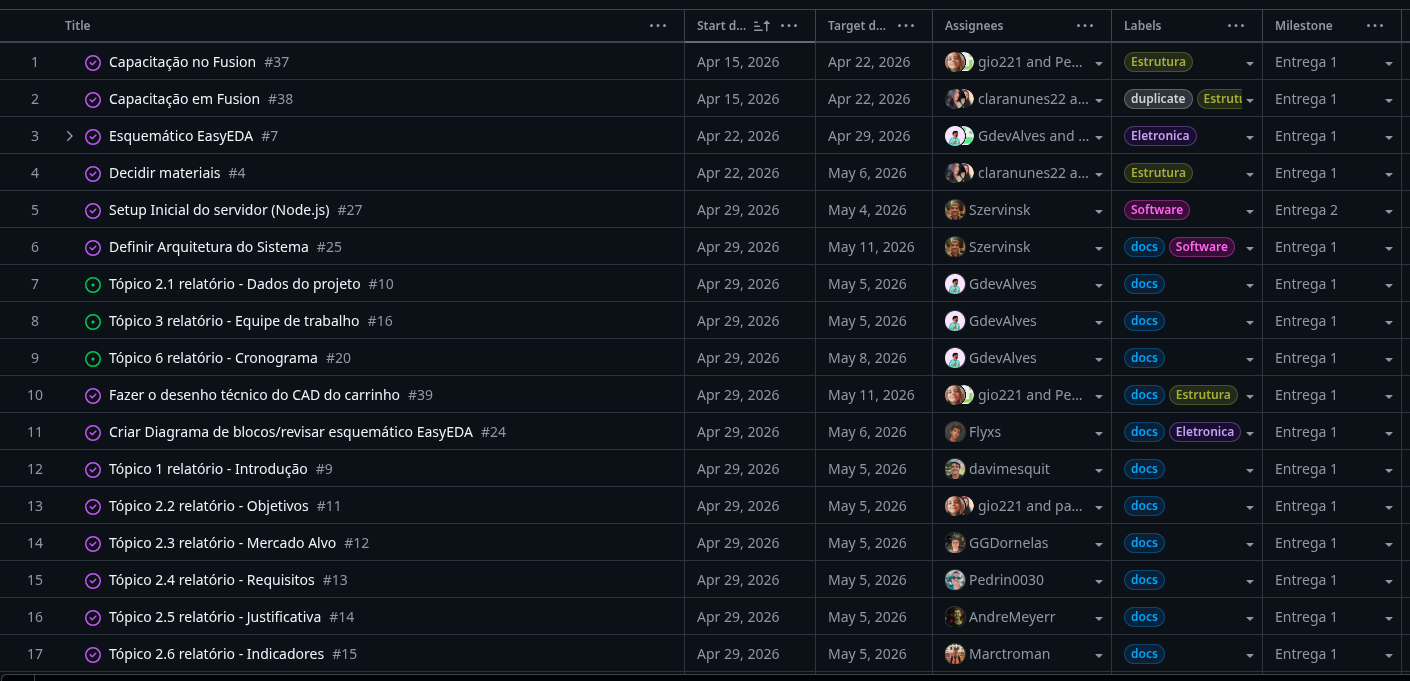
\includegraphics[width=\linewidth]{figuras/1-17.png}
    \caption{}
    \label{fig:cronograma_1_17}
\end{figure}
\end{landscape}

\begin{landscape}
\begin{figure}[H]
    \centering
    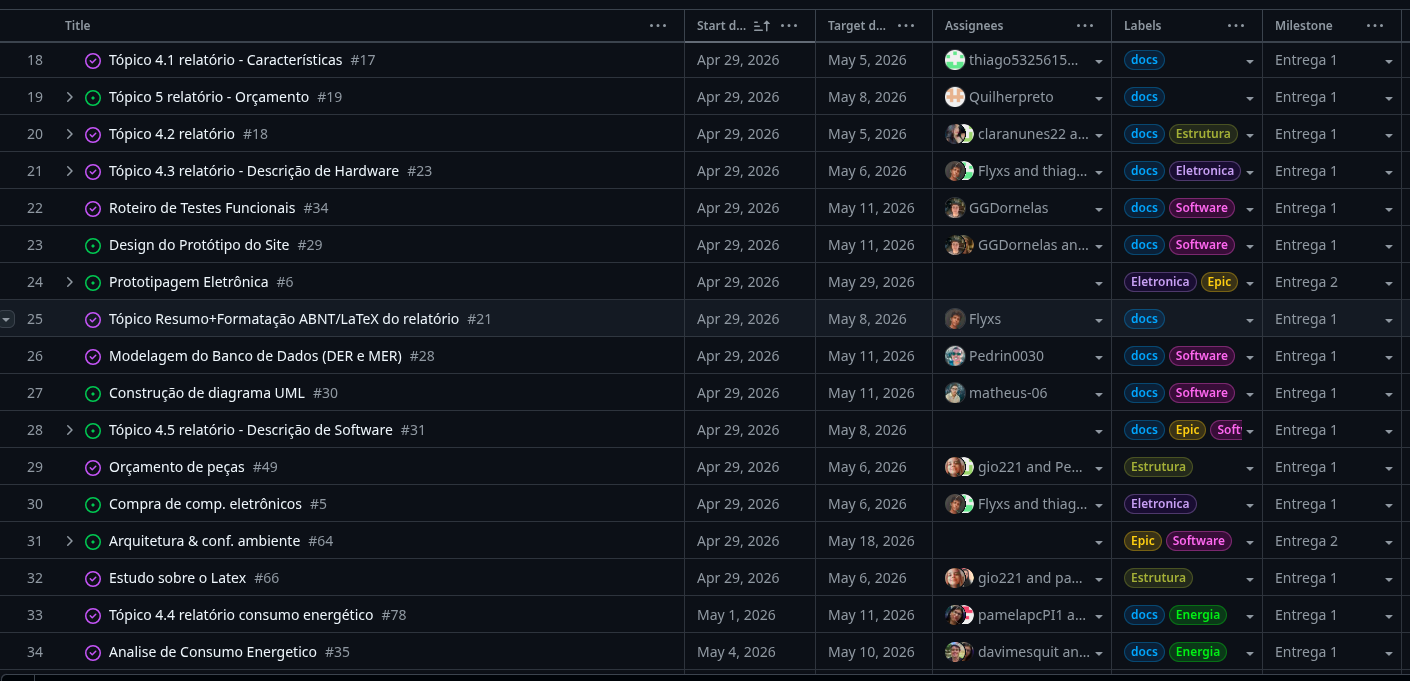
\includegraphics[width=\linewidth]{figuras/18-34.png}
    \caption{}
    \label{fig:cronograma_18_34}
\end{figure}
\end{landscape}

\begin{landscape}
\begin{figure}[H]
    \centering
    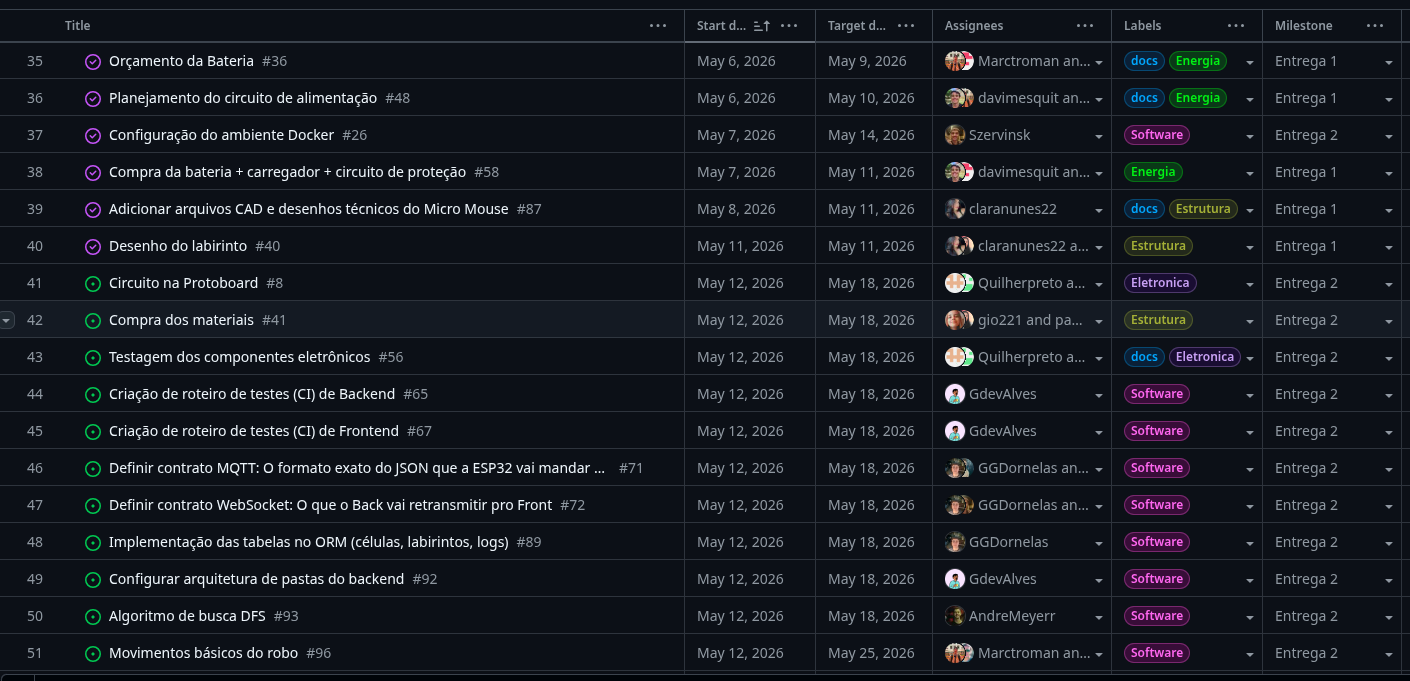
\includegraphics[width=\linewidth]{figuras/35-51.png}
    \caption{}
    \label{fig:cronograma_35_51}
\end{figure}
\end{landscape}

\begin{landscape}
\begin{figure}[H]
    \centering
    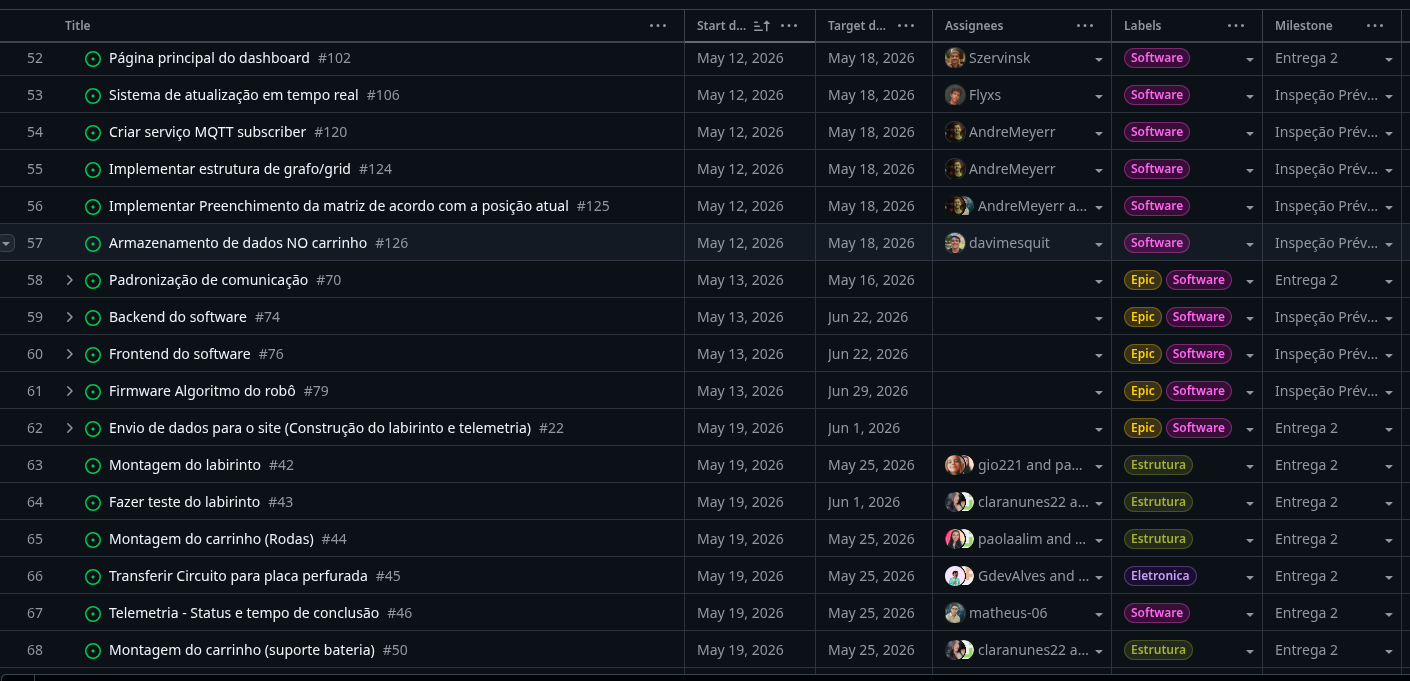
\includegraphics[width=\linewidth]{figuras/52-68.png}
    \caption{}
    \label{fig:cronograma_52_68}
\end{figure}
\end{landscape}

\begin{landscape}
\begin{figure}[H]
    \centering
    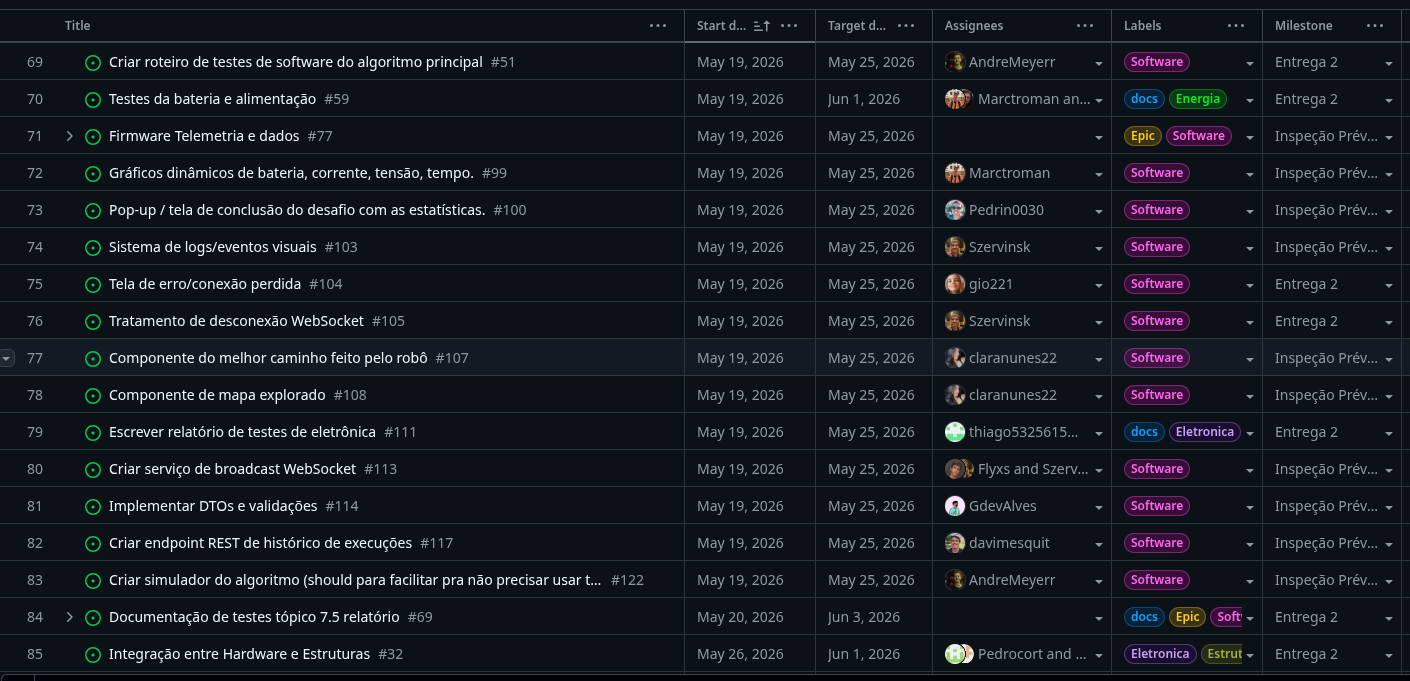
\includegraphics[width=\linewidth]{figuras/69-85.png}
    \caption{}
    \label{fig:cronograma_69_85}
\end{figure}
\end{landscape}

\begin{landscape}
\begin{figure}[H]
    \centering
    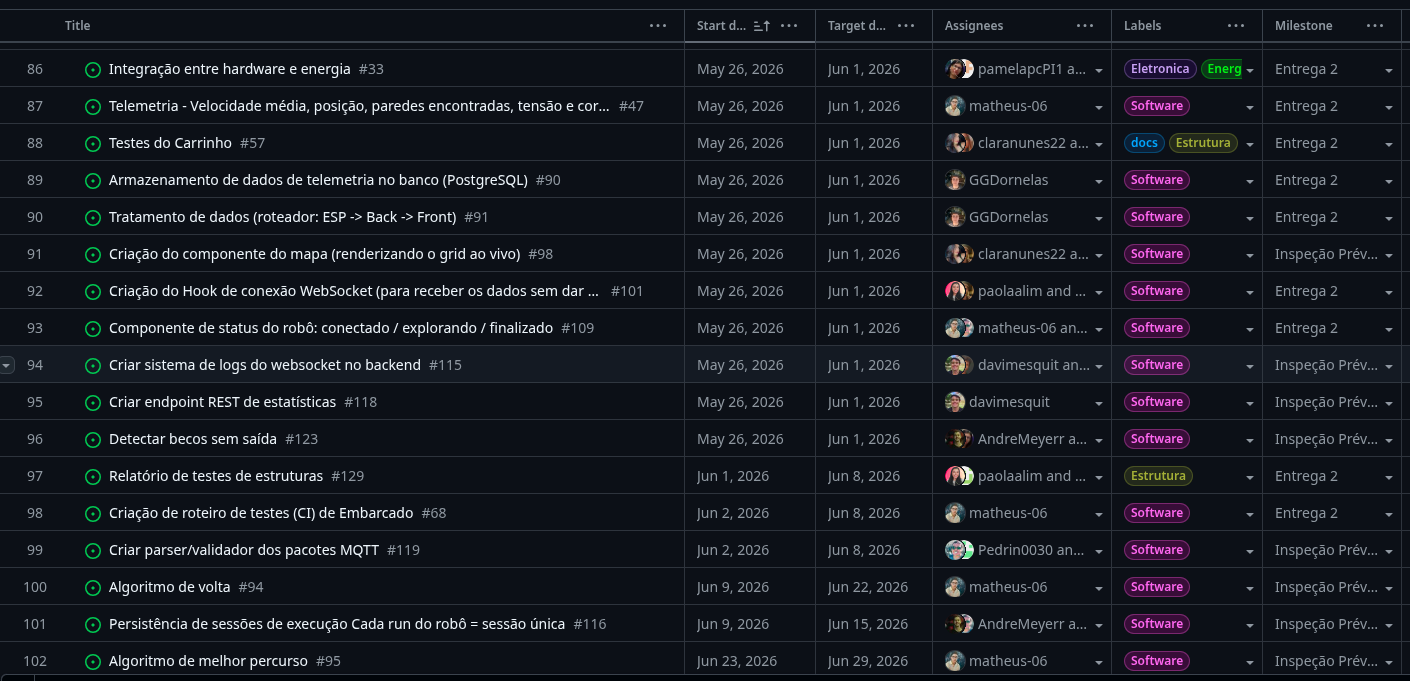
\includegraphics[width=\linewidth]{figuras/86-102.png}
    \caption{}
    \label{fig:cronograma_86_102}
\end{figure}
\end{landscape}

\begin{landscape}
\begin{figure}[H]
    \centering
    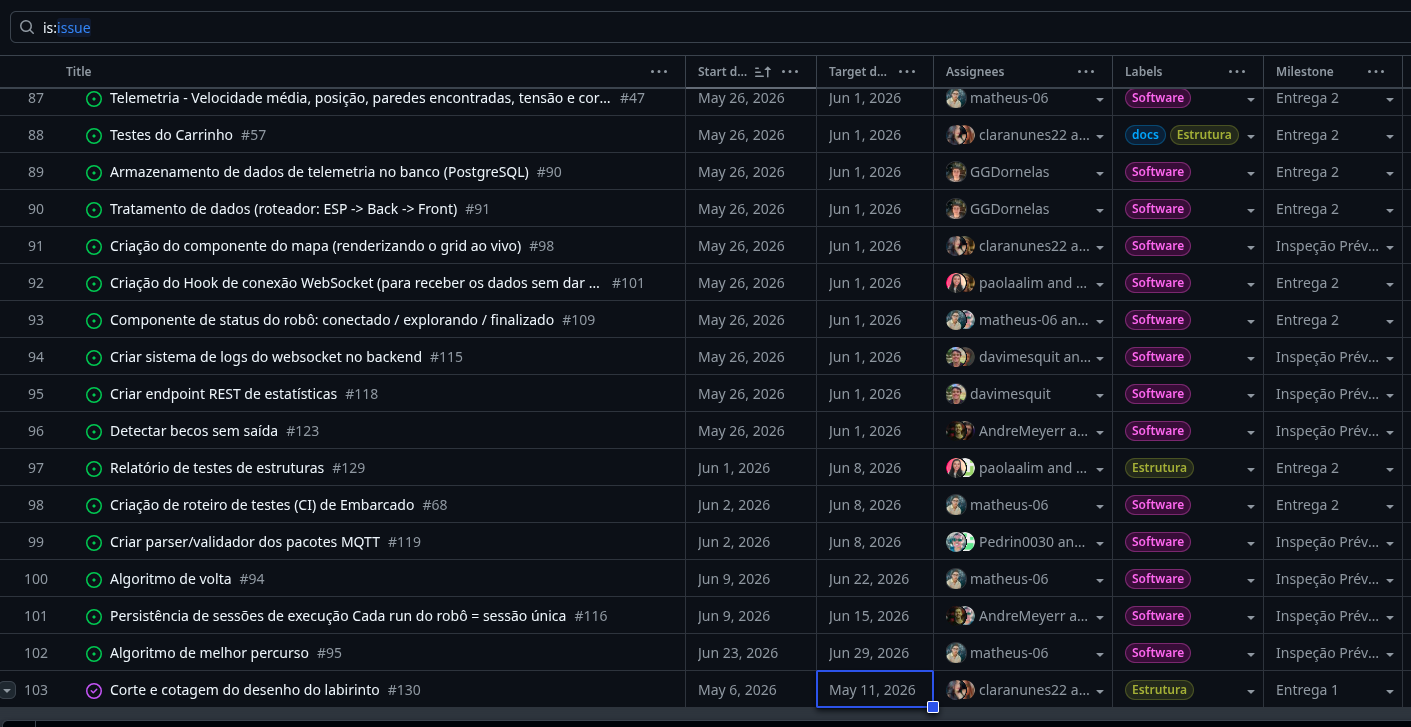
\includegraphics[width=\linewidth]{figuras/103.png}
    \caption{}
    \label{fig:cronograma_103}
\end{figure}
\end{landscape}


% \begin{table}[htpb]
% \begin{center}
% \caption{Cronograma por atividade.}
% \begin{tabular}{|c|c|c|c|c|c|c|}
% \hline
% & \textbf{Início} & \textbf{Início} & \textbf{Fim} & \textbf{Fim} & \textbf{Atividades} & \\
% \textbf{Atividade} & \textbf{Previsto} & \textbf{Realizado} & \textbf{Previsto} & \textbf{Realizado} & \textbf{Predecessoras} & \textbf{Responsáveis}\\ \hline
% 1 - ABC                       & DD/MM/AAAA               & DD/MM/AAAA                & DD/MM/AAAA               & DD/MM/AAAA                & ---                               & Fulano \\ \hline
% 2 - DEF                       & DD/MM/AAAA               & DD/MM/AAAA                & DD/MM/AAAA               & DD/MM/AAAA                & 1                                 & Fulano \\ \hline
% 3 - GHI                       & DD/MM/AAAA               & DD/MM/AAAA                & DD/MM/AAAA               & DD/MM/AAAA                & 1, 2                              & Beltrano \\ \hline
% 4 - JKL                       & DD/MM/AAAA               & DD/MM/AAAA                & DD/MM/AAAA               & DD/MM/AAAA                & 3                                 & Beltrano \\ \hline
% 5 - MNO                       & DD/MM/AAAA               & DD/MM/AAAA                & DD/MM/AAAA               & DD/MM/AAAA                & 1, 3, 4                           & Ciclano \\ \hline
% \end{tabular}
% \end{center}
% \end{table}



% \begin{table}[htpb]
% \begin{center}
% \caption{Justificativas para atrasos ou não-conclusão de atividades.}
% \begin{tabular}{|c|c|} \hline
% \textbf{Atividade} & \textbf{Justificativa}  \\ \hline 
%     3 - GHI &
%     O material solicitado não foi entregue no prazo pelo fornecedor. \\ \hline
%     5 - MNO &
%     A equipe responsável pelo desenvolvimento não finalizou a atividade. \\ \hline
% \end{tabular}
% \end{center}
% \end{table}

% %% Exemplo de tabela que ocupa várias páginas
% \begin{center}
% \begin{longtable}{|l|l|l|}
% \caption{A sample long table.} \label{tab:long} \\

% \hline \multicolumn{1}{|c|}{\textbf{First column}} & \multicolumn{1}{c|}{\textbf{Second column}} & \multicolumn{1}{c|}{\textbf{Third column}} \\ \hline 
% \endfirsthead

% \multicolumn{3}{c}%
% {{\bfseries \tablename\ \thetable{} -- continued from previous page}} \\
% \hline \multicolumn{1}{|c|}{\textbf{First column}} & \multicolumn{1}{c|}{\textbf{Second column}} & \multicolumn{1}{c|}{\textbf{Third column}} \\ \hline 
% \endhead

% \hline \multicolumn{3}{|r|}{{Continued on next page}} \\ \hline
% \endfoot

% \hline \hline
% \endlastfoot

% One & abcdef ghjijklmn & 123.456778 \\
% One & abcdef ghjijklmn & 123.456778 \\
% One & abcdef ghjijklmn & 123.456778 \\
% One & abcdef ghjijklmn & 123.456778 \\
% One & abcdef ghjijklmn & 123.456778 \\
% One & abcdef ghjijklmn & 123.456778 \\
% One & abcdef ghjijklmn & 123.456778 \\
% \end{longtable}
% \end{center}
\chapter{Testes de Verificação e Validação}

\section{Características Gerais}

\section{Testes da estrutura}

\section{Testes de \textit{hardware}}


\section{Testes de consumo energético}


\section{Testes de \textit{software}}


\section{Testes de integração}


\chapter{Lições Aprendidas}

\section{Análise SWOT}


\begin{table}[ht]
% \label{tab:swot}
\centering
\caption{Análise SWOT do produto.}
\begin{tabular}{|c|c|c|} \hline
 & \textbf{Pontos fortes} & \textbf{Pontos fracos}  \\ \hline 
    {\parbox{0.1\textwidth}{ \textbf{Fatores \\ internos}}}  &
    {\parbox{0.4\textwidth}{ Forças: 
       \begin{itemize}
            \item Lorem ipsum
            \item Lorem ipsum
        \end{itemize} }} & 
    {\parbox{0.4\textwidth}{ Fraquezas:
        \begin{itemize}
            \item Lorem ipsum
            \item Lorem ipsum
        \end{itemize} }}\\ \hline
    {\parbox{0.1\textwidth}{ \textbf{Fatores \\ externos}}}  &
    {\parbox{0.4\textwidth}{ Oportunidades:
        \begin{itemize}
            \item Lorem ipsum 
            \item Lorem ipsum
        \end{itemize} }} & 
    {\parbox{0.4\textwidth}{ Ameaças:
         \begin{itemize}
            \item Lorem ipsum 
            \item Lorem ipsum
        \end{itemize} }}\\ \hline
\end{tabular}
\label{tab:swot}
\end{table}


\section{Planejado x realizado}
\subsection{Objetivos}
\subsection{Prazos}
\subsection{Orçamento}
\subsection{Escopo}


\section{Projeto}
\subsection{Pontos fortes}

\subsection{Pontos fracos}

\section{Recomendações para projetos futuros}



\section{Questões em aberto}



\section{Desempenho dos fornecedores}

\subsection{Fornecedores com desempenho acima do esperado}

\subsection{Fornecedores com desempenho conforme esperado}

\subsection{Fornecedores com desempenho abaixo do esperado}


% ----------------------------------------------------------
% ELEMENTOS PÓS-TEXTUAIS
% ----------------------------------------------------------
\bookmarksetup{startatroot} % Destrava os marcadores do sumário para os apêndices

\postextual

\bibliography{bibliografia}
% \begin{apendicesenv}
% \partapendices

% \chapter{Primeiro Apêndice}


%%% https://www.codecogs.com/latex/eqneditor.php?lang=pt-br
% \begin{equation}
%     \alpha = \sum_{i=0}^{\infty}{a_i x^i}
% \end{equation}

% \begin{equation}
%     \beta = \sum_{i=0}^{\infty}{a_i x^{2\pi i}\frac{\partial^2 }{\partial x^2}}f(xi)
% \end{equation}





% \chapter{Segundo Apêndice}




% \end{apendicesenv}
\begin{anexosenv}
% \partanexos

\chapter{Primeiro Anexo}


\chapter{Segundo Anexo}

\begin{figure}[htpb]
\centering

\includegraphics[width=\textwidth]{figuras/fga.png}
\caption{Figura do Anexo 2.}
\label{fig:fig_anexo}
\end{figure}

\end{anexosenv}

\printindex

\end{document}